\documentclass[a4paper,11pt]{article}
\usepackage{lecturenotes}
\usepackage{enumitem}
\setlist{itemsep=2pt,parsep=0pt,topsep=4pt}
\raggedbottom
\widowpenalty=10000
\clubpenalty=10000
\lstset{basicstyle=\fontsize{9.5}{11}\selectfont\ttfamily\color{NoteInk}}
\lectureheader{COE718}{4}
\fancyfoot[C]{\sffamily\small\color{NoteMuted}\thepage}
\newcommand{\code}[1]{\texttt{#1}}
\newsavebox{\fcfsimagebox}
\newlength{\fcfstoptrim}
\newcommand{\sourcefigure}[2]{%
  \par\smallskip\noindent\begin{minipage}{\linewidth}\centering
  \includegraphics[width=\linewidth,height=#2,keepaspectratio]{figures/#1}\par
  \end{minipage}\par\smallskip}
\begin{document}
\tableofcontents
\clearpage
\notesection{Operating Systems and Processes}



An OS must interleave the execution of several processes to maximize CPU usage, must allocate resources to processes (CPU, Memory, I/O, WIFI, etc), and must support \emph{interprocess communication} (Shared memory, ports, etc).\par



\textbf{Operating System:} Provides a SW layer over hardware and has three primary functions: 1. Schedule task execution 2. Dispatch a task for execution, and 3. Ensure communication and synchronization between tasks\par



\subnotesection{Concurrency}



Only \emph{one thread} runs while others are waiting. The processor switches from one process to another so quickly that it appears that all threads are running simultaneously. This is called \emph{concurrency}. The programmer assigns a priority to each process, and the scheduler uses that to determine which process to run next\par



\textbf{Concurrency:} The appearance of simultaneous execution of multiple tasks\par

\noteheading{3}{Real-time Kernel}



Processes call a library of run-time routines to manage resources. The kernel provides mechanisms to switch between processes for coordination, synchronization, communication, and priority.\par



\sourcefigure{image-00930.png}{108mm}

\Needspace{125pt}
\notesection{Basic Process States}



\Needspace{52pt}
\begin{multicols}{2}
\begin{itemize}
\item \begin{minipage}[t]{\linewidth}\textbf{Running State:} The process that gets executed\end{minipage}
\item \begin{minipage}[t]{\linewidth}\textbf{Ready State:} A process that is ready to be executed\end{minipage}
\item \begin{minipage}[t]{\linewidth}\textbf{Blocked State (Waiting):} When a process cannot execute until some event occurs\end{minipage}
\end{itemize}
\end{multicols}

\subnotesection{Modes of Execution}



Most processors support at-least two execution modes\par



\textbf{Privileged}: Allows manipulation of control registers, memory, etc.\par

\textbf{User Mode}: Less privileged, applications execute in this mode.\par



The CPU provides one or more \emph{mode bits}, and they can only be set by an interrupt or trap or OS call.\par



\sourcefigure{image-01517.png}{100mm}

\subnotesection{Unix Processes}



There exists two modes: user mode and kernel mode. System (OS) processes run in kernel mode. User processes run in user mode for user instructions, and in kernel mode for OS/kernel instructions.\par



There is \emph{9 states for processes}\par



\textbf{Unix Process States}\par

\Needspace{52pt}
\begin{itemize}
\item There is two running states for user or kernel modes
\item Pre-empted state is for processes returning from Kernel to user mode. A process running Kernel mode cannot be pre-empted. \textbf{This makes Linux unsuitable for real-time applications}
\end{itemize}



\Needspace{140pt}
\noteheading{3}{UNIX Process Creation}



Every process, except process 0, is created by a \textbf{fork()} syscall.\par

\Needspace{76pt}
\begin{itemize}
\item \textbf{fork():} allocates an entry into the process table and assigns a unique PID (process ID) to the child process.
\begin{itemize}
\item A child gets a copy of the process/task image of parent - both child and parent are executing the same code following the \emph{fork()}
\item Returns the PID of the child to the parent process and returns 0 to the child process
\end{itemize}
\end{itemize}



Process 0 is created at boot time and becomes the \emph{"swapper"} after forking process 1 (\textbf{INIT Process}). I.e. when a user logs in, process 1 creates a process for that user.\par



\noteheading{3}{UNIX-style Process Creation}



\begingroup\small
\begin{notetable}{@{}>{\raggedright\arraybackslash}p{0.38\linewidth}>{\raggedright\arraybackslash}X@{}}{\textbf{Call} & \textbf{Description}}
\code{pid = fork()} & Create a child process identical to the parent \\
\code{pid = waitpid(pid, \&statloc, options)} & Wait for a child to terminate; blocks itself \\
\code{s = execve(name, argv, environp)} & Replace a process's core image \\
\code{exit(status)} & Terminate process execution and return status \\
\end{notetable}
\endgroup



\Needspace{395pt}
\noteheading{4}{Example UNIX Fork Example}



\begin{minipage}{\linewidth}
\begin{notecode}[language=C,basicstyle=\fontsize{9.5}{11}\selectfont\ttfamily\color{NoteInk}]
#include <sys/types.h>
#include <stdio.h>
#include <unistd.h>

int main()
{
    pid_t pid;

    pid = getpid();  /* Parent process created, get its ID */
    pid = fork();    /* Create a child process */

    if (pid == 0)
    {
        /* Only the child process code should get here */
        while (1)
        {
            fprintf(stderr, "I am child process\n");
            usleep(10000000);  /* Wait for 10 seconds */
        }
    }

    /* Only the parent should get here */
    fprintf(stderr, "I am PARENT: I wait for 20 seconds\n");
    usleep(20000000);

    fprintf(stderr, "I am PARENT: Kill child: %u\n", pid);
    kill(pid, 9);

    return 0;
}
\end{notecode}
\end{minipage}



\sourcefigure{image-02436.png}{105mm}

\subnotesection{Process Context and Switching}



Each process has its own stack and context. A \emph{context switch} from process "A" to process "B" first saves registers in context A, then reloads all CPU registers from context B.\par

\Needspace{125pt}
\noteheading{3}{Process/Task Switching}



\begin{enumerate}
\item Save context of processor (PC and other registers)
\item Update the PCB/TCB (process/task control block) with the new state and other associated information
\item Move PCB to appropriate queue
\item Select another process for execution
\item Update the process (task) control block of the process (task) selected
\item Update memory-management data structures
\item Restore context of the selected process by reloading previous PC and registers
\end{enumerate}



\sourcefigure{image-03443.png}{120mm}

\subnotesection{Foreground/Background System}





Most of actual work is performed in "foreground" ISRs, with each ISR processing a particular hardware event. The main program performs initialization, and enters a background event \emph{waiting for interrupts to occur}\par



The system responds to external events with a predictable amount of latency.\par



\textbf{Moving to the Background}\par



We can instead move non-time critical work (such as updating a display) into a background task. The foreground ISR writes data to queue, then background removes the data and processes it. An alternative to ignoring one or more interrupts as a result of \emph{input overrun}\par



\Needspace{125pt}
\noteheading{3}{Limitations}



\Needspace{64pt}
\begin{multicols}{2}
\begin{itemize}
\item \begin{minipage}[t]{\linewidth}Best possible performance requires moving as much as possible into the background\end{minipage}
\item \begin{minipage}[t]{\linewidth}The background then becomes a collection of queues and associated routines to process said data\end{minipage}
\item \begin{minipage}[t]{\linewidth}Optimizes latency of individual ISRs, but the background requires a managed allocation of processor time\end{minipage}
\end{itemize}
\end{multicols}



It is good for smaller applications that have no need of an OS\par



\sourcefigure{image-04246.png}{100mm}

\subnotesection{Cooperative Multitasking}



It hides the context switching mechanism but still relies on processes to give up CPU use. Each process allows a context switch at \textbf{cswitch()} call. A separate scheduler chooses which process runs next.\par



\textbf{Context Switching:} Controls when the context is switched (user/code), and how it is switched\par



\Needspace{140pt}
\noteheading{3}{Limitations}



Programming errors (code errors) can keep other processes out:\par

\Needspace{40pt}
\begin{itemize}
\item Process never gives up the CPU
\item Process waits too long to switch, and misses input
\end{itemize}



\subnotesection{Preemptive Multi-tasking}



Is the most powerful form of multi-tasking. The OS controls when the context switches and determines which process to run next. Uses a timer to call OS, and switch contexts.\par



\emph{Is the most widely method for RT embedded systems}\par



\subnotesection{VxWorks Multitasking}



Modern systems use a mix of multi-tasking and intertask communication. Tasks have immediate, shared access to most system resources while maintaining separate context to maintain individual task control. A multi-tasking environment allows a RT app to be constructed as a set of independent tasks each with its own thread of execution and set of sys resources (\emph{No priority inversion})\par



\Needspace{135pt}
A VxWorks Task Context has:\par

\begin{multicols}{2}
\begin{itemize}
\item \begin{minipage}[t]{\linewidth}a thread of execution (function/code) (task's program counter)\end{minipage}
\item \begin{minipage}[t]{\linewidth}CPU registers and optionally floating-point registers\end{minipage}
\item \begin{minipage}[t]{\linewidth}A stack for dynamic variables and function calls\end{minipage}
\item \begin{minipage}[t]{\linewidth}I/O assignments for standard input, output and error\end{minipage}
\item \begin{minipage}[t]{\linewidth}A delay timer\end{minipage}
\item \begin{minipage}[t]{\linewidth}A time-slice timer\end{minipage}
\item \begin{minipage}[t]{\linewidth}Kernel Control Structures\end{minipage}
\item \begin{minipage}[t]{\linewidth}Signal handler\end{minipage}
\item \begin{minipage}[t]{\linewidth}Debugging and performance monitoring values\end{minipage}
\end{itemize}
\end{multicols}



An important resource that is \emph{not} a part of a task's context in memory address space. All code executes in a single common address space.\par



\notesection{RTX - RTOS Kernel}



The RTX kernel is a realtime operating system (RTOS)\par



RTX stands for: Real Time eXecutive for microcontrollers based on ARM CPU cores\par



Its basic functionality is to start and stop concurrent tasks (processes, and has functionality for Inter Process Communication (IPC):\par

\Needspace{52pt}
\begin{multicols}{2}
\begin{itemize}
\item \begin{minipage}[t]{\linewidth}Synchronize different tasks\end{minipage}
\item \begin{minipage}[t]{\linewidth}Manage common resources (peripherals or memory regions)\end{minipage}
\item \begin{minipage}[t]{\linewidth}Pass complete messages between tasks\end{minipage}
\end{itemize}
\end{multicols}



\textbf{Advantages:}\par

\Needspace{64pt}
\begin{multicols}{2}
\begin{itemize}
\item \begin{minipage}[t]{\linewidth}Tasks can be prioritized\end{minipage}
\item \begin{minipage}[t]{\linewidth}Splitting up the application software into independent parts reduces the systems complexity, errors, and may facilitate testings\end{minipage}
\item \begin{minipage}[t]{\linewidth}RTX kernel is scalable as additional tasks can be added easily at a later time\end{minipage}
\end{itemize}
\end{multicols}



The RTX is a royalty free deterministic RTOS with:\par

\Needspace{76pt}
\begin{multicols}{2}
\begin{itemize}
\item \begin{minipage}[t]{\linewidth}Round-robin, pre-emptive and collaborative scheduling\end{minipage}
\item \begin{minipage}[t]{\linewidth}Small footprint for resource constrained systems\end{minipage}
\item \begin{minipage}[t]{\linewidth}Unlimited number of tasks each with 254 priority levels\end{minipage}
\item \begin{minipage}[t]{\linewidth}Unlimited number of mailboxes, semaphores, mutex, and timers\end{minipage}
\item \begin{minipage}[t]{\linewidth}Supports multi-threading\end{minipage}
\end{itemize}
\end{multicols}



\Needspace{140pt}
\subnotesection{Keils RTS for ARM CPUs}



The \textless{}RTL.h\textgreater{} file defines the RTX functions and macros. Offers interrupt handling, multitasking, periodic task activations, and scalable task creation. Uses \code{RTX\_Config\_CM.c} to specify parameters and configuration in the RTOS/RTX kernel\par

\Needspace{40pt}
\begin{itemize}
\item Ports the kernel to the CPU
\item Includes \emph{cmis\_os.h}, which provides access to the CMSIS\_RTOS\_API
\end{itemize}



\subnotesection{RTX Multitasking}



The RTOS enables us to create applications that can perform multiple functions or tasks, and flexible scheduling of system resources like CPU and memory, and offers ways/supports to communicate between tasks\par



\begingroup\small
\begin{notetable}{@{}>{\raggedright\arraybackslash}p{0.38\linewidth}>{\raggedright\arraybackslash}X>{\raggedright\arraybackslash}X@{}}{\textbf{Description} & \textbf{ARM7 / ARM9} & \textbf{Cortex-M}}
RAM space for kernel & 300 bytes + 80-byte user stack & 300 bytes + 128-byte main stack \\
Hardware requirements & One on-chip timer & SysTick timer \\
Context switch time & \textless{} 5.3 $\mu$s at 60 MHz & \textless{} 2.6 $\mu$s at 72 MHz \\
\end{notetable}
\endgroup



\textbf{Timing Specifications}\par



\begingroup\small
\begin{notetable}{@{}>{\raggedright\arraybackslash}p{0.38\linewidth}>{\raggedright\arraybackslash}X>{\raggedright\arraybackslash}X@{}}{\textbf{Function} & \textbf{ARM7 / ARM9 (cycles)} & \textbf{Cortex-M (cycles)}}
Cooperative task switch (\code{os\_tsk\_pass}) & 321 & 192 \\
\end{notetable}
\endgroup



\Needspace{395pt}
\noteheading{3}{Task Creation Example}



\begin{minipage}{\linewidth}
\begin{notecode}[language=C,basicstyle=\fontsize{9.5}{11}\selectfont\ttfamily\color{NoteInk}]
#include <RTL.h>       /* RTX header file for RTX system calls */
#include <LPC17xx.H>   /* LPC17xx Cortex-M3 board definitions */

long global_c1 = 0, global_c2 = 0;

__task void task1(void)
{
    for (;;)
    {
        global_c1 += 3;
    }
}

__task void task2(void)
{
    for (;;)
    {
        global_c2 += 2;
    }
}

int main(void)
{
    SystemInit();                 /* Initialize the Cortex-M3 processor */
    os_tsk_create(task1, 1);       /* Create task1 with priority 1 */
    os_tsk_create(task2, 1);       /* Create task2 with priority 1 */
    os_tsk_delete_self();         /* Kill itself; task1 starts */

    os_sys_init(task1);            /* Initialize RTX and start task1 */
}
\end{notecode}
\end{minipage}

\Needspace{260pt}
\noteheading{3}{Task States and Management}



Each RTX task is always in \textbf{one state},\par



\textbf{RUNNING:} The task that is currently running is in the \code{RUNNING} state. Only one task at a time can be in this state\par



\textbf{READY:} Tasks which are ready to run are in the \code{READY} state. Once the running task has completed processing, RTX selects the next ready task with the \textbf{highest priority} and starts it\par



\textbf{WAIT\_DLY:} Tasks that are waiting for a delay to expire are in the \code{WAIT\_DLY} state. Once the delay has expired, the task is switched to the \code{READY} state\par

\Needspace{112pt}
\begin{itemize}
\item \textbf{WAIT\_ITV:} Tasks waiting for an interval to expire. Once the delay has expired, the task is switched back to the \code{READY} state. Uses \code{os\_itv\_wait()}
\item \textbf{WAIT\_SEM:} Tasks waiting for a semaphore. When the token is obtained from the semaphore, the task is switched back to the \code{READY} state. Uses \code{os\_sem\_wait()}
\item \textbf{WAIT\_MUT:} Tasks waiting for a free mutex. When it is released, the task acquires the mutex and is switched to the \code{READY} state. Uses \code{os\_mut\_wait()}
\item \textbf{INACTIVE:} Tasks that are not started or have been deleted. \code{os\_task\_delete()} places a task that has been started (with \code{os\_tsk\_create()} into the \code{INACTIVE} state
\end{itemize}



\begingroup\small
\begin{notetable}{@{}>{\raggedright\arraybackslash}p{0.38\linewidth}>{\raggedright\arraybackslash}X@{}}{\textbf{Routine} & \textbf{Description}}
\code{os\_sys\_init} & Initializes and starts RL-RTX. \\
\code{os\_sys\_init\_prio} & Initializes and starts RL-RTX, assigning a priority to the starting task. \\
\code{os\_sys\_init\_user} & Initializes and starts RL-RTX, assigning a priority and custom stack to the starting task. \\
\code{os\_tsk\_create} & Creates and starts a new task. \\
\code{os\_tsk\_create\_ex} & Creates and starts a new task, passing it an argument pointer. \\
\code{os\_tsk\_create\_user} & Creates and starts a new task with a custom stack. \\
\code{os\_tsk\_create\_user\_ex} & Creates and starts a new task with a custom stack, passing it an argument pointer. \\
\code{os\_tsk\_delete} & Stops and deletes a task. \\
\code{os\_tsk\_delete\_self} & Stops and deletes the currently running task. \\
\code{os\_tsk\_pass} & Passes control to the next task of the same priority. \\
\code{os\_tsk\_prio} & Changes a task's priority. \\
\code{os\_tsk\_prio\_self} & Changes the currently running task's priority. \\
\code{os\_tsk\_self} & Obtains the task ID of the currently running task. \\
\code{isr\_tsk\_get} & Obtains the task ID of the interrupted task. \\
\end{notetable}
\endgroup



\notesection{CMSIS}



\textbf{CMSIS:} Cortex Microcontroller Software Interface Standard. A \emph{Device Driver Library} providing an independent HW abstraction layer for interfacing applications to the microcontroller.\par



\sourcefigure{image-11613.png}{110mm}

\begingroup\small
\begin{notetable}{@{}>{\raggedright\arraybackslash}p{0.38\linewidth}>{\raggedright\arraybackslash}X@{}}{\textbf{Routine} & \textbf{Description}}
\code{osKernelInitialize} & Initializes the RTOS kernel. \\
\code{osKernelStart} & Starts the RTOS kernel. \\
\code{osKernelGetState} & Gets the current RTOS kernel state. \\
\code{osKernelGetSysTimerCount} & Gets the RTOS kernel system timer count. \\
\code{osKernelSuspend} & Suspends the RTOS kernel scheduler. \\
\code{osKernelResume} & Resumes the RTOS kernel scheduler. \\
\code{osDelay} & Waits for a timeout (time delay). \\
\code{osThreadCreate} & Creates and starts a new thread, passing it an argument pointer. \\
\code{osThreadTerminate} & Stops and deletes a thread. \\
\code{osThreadYield} & Passes control to the next thread. \\
\code{osThreadSetPriority} & Changes a thread's priority. \\
\code{osThreadGetPriority} & Gets a thread's priority. \\
\code{osThreadGetId} & Obtains the ID of the currently running thread. \\
\code{osSemaphoreCreate} & Defines and initializes a semaphore. \\
\code{osSemaphoreWait} & Obtains a semaphore token or waits until one becomes available. \\
\code{osSemaphoreRelease} & Releases a semaphore token. \\
\code{osSemaphoreDelete} & Deletes a semaphore. \\
\end{notetable}
\endgroup

\Needspace{373pt}
\subnotesection{Thread Creation and Execution (Example - Round Robin Scheduling)}



\begin{minipage}{\linewidth}
\begin{notecode}[language=C,basicstyle=\fontsize{9.5}{11}\selectfont\ttfamily\color{NoteInk}]
#include "cmsis_os.h"

unsigned int global_c1 = 0, global_c2 = 0;
osThreadId tid_Thread, tid2_Thread;

void Thread1(void const *argument) {
    for (;;) global_c1 += 3;
}
void Thread2(void const *argument) {
    for (;;) global_c2 += 2;
}

// Both threads have the same priority.
osThreadDef(Thread1, osPriorityNormal, 1, 0);
osThreadDef(Thread2, osPriorityNormal, 1, 0);

int Init_Thread(void) {
    tid_Thread  = osThreadCreate(osThread(Thread1), NULL);
    tid2_Thread = osThreadCreate(osThread(Thread2), NULL);
    return (!tid_Thread || !tid2_Thread) ? -1 : 0;
}

int main(void) {
    osKernelInitialize();
    Init_Thread();
    osKernelStart();
    osDelay(osWaitForever);
}
\end{notecode}
\end{minipage}

\Needspace{140pt}
\subnotesection{RTX: Cooperative Multi-tasking}



We can design and implement tasks so they execute cooperatively. Specifically, we must call sys wait functions such as: \code{os\_dly\_wait()} or \code{os\_tsk\_pass()} somewhere in each task. These functions signal the RTX kernel to switch.\par

\Needspace{64pt}
\begin{itemize}
\item \code{os\_dly\_wait()}: Allows task to wait for an event
\item \code{os\_tsk\_pass()}: Switches to another ready task immediately. If the next ready task has a lower priority than the currently running task, then calling this method does not cause a task switch 
\end{itemize}



\Needspace{100pt}
The following example:\par

\Needspace{64pt}
\begin{multicols}{2}
\begin{itemize}
\item \begin{minipage}[t]{\linewidth}Has an RTX kernel starts executing task1 that creates task2\end{minipage}
\item \begin{minipage}[t]{\linewidth}After counter1 is incremented, the kernel switches to task2\end{minipage}
\item \begin{minipage}[t]{\linewidth}After counter2 is incremented, the kernel switches back to task1. This process repeats indefinitely\end{minipage}
\end{itemize}
\end{multicols}



\Needspace{329pt}
\noteheading{3}{RTX Cooperative Multitasking Example}



\begin{minipage}{\linewidth}
\begin{notecode}[language=C,basicstyle=\fontsize{9.5}{11}\selectfont\ttfamily\color{NoteInk}]
#include <rtl.h>

int counter1, counter2;
__task void task2(void);

__task void task1(void) {
    os_tsk_create(task2, 0);  // Create task2 and mark it ready
    for (;;) {
        counter1++;
        os_tsk_pass();       // Yield to task2
    }
}

__task void task2(void) {
    for (;;) {
        counter2++;
        os_tsk_pass();       // Yield to task1
    }
}

void main(void) {
    os_sys_init(task1);      // Initialize RTX and start task1
    for (;;);
}
\end{notecode}
\end{minipage}



\Needspace{483pt}
\noteheading{3}{Threads and Cooperative Multitasking Example}

\begin{minipage}{\linewidth}
\begin{notecode}[language=C,basicstyle=\fontsize{9.5}{11}\selectfont\ttfamily\color{NoteInk}]
#include "cmsis_os.h"

unsigned int counter1, counter2;
osThreadId tid_Thread, tid2_Thread;

void Thread1(void const *argument) {
    osStatus status;
    for (;;) {
        counter1++;
        status = osThreadYield();
        if (status != osOK) { /* Handle yield failure */ }
    }
}

void Thread2(void const *argument) {
    osStatus status;
    for (;;) {
        counter2++;
        status = osThreadYield();
        if (status != osOK) { /* Handle yield failure */ }
    }
}

osThreadDef(Thread1, osPriorityNormal, 1, 0);
osThreadDef(Thread2, osPriorityNormal, 1, 0);

int Init_Thread(void) {
    tid_Thread  = osThreadCreate(osThread(Thread1), NULL);
    tid2_Thread = osThreadCreate(osThread(Thread2), NULL);
    return (!tid_Thread || !tid2_Thread) ? -1 : 0;
}

int main(void) {
    osKernelInitialize();
    Init_Thread();
    osKernelStart();
    osDelay(osWaitForever);
}
\end{notecode}
\end{minipage}



\Needspace{140pt}
\notesection{IPC: Interprocess Communication}



Two types of semantics for data-passing between processes\par

\Needspace{40pt}
\begin{itemize}
\item \textbf{Blocking:} The sending process waits for a response
\item \textbf{Non-blocking:} The sending process continues to execute
\end{itemize}



\Needspace{100pt}
\subnotesection{IPC Styles}



\textbf{Shared Memory:} Processes have some memory in common. They must cooperate to avoid destroying/missing any messages\par

\textbf{Message Passing:} Processes send messages along a common communication channel, and have no common address space\par



\notesection{Critical Regions}



\textbf{Critical Region:} Section of code that cannot be interrupted by another process i.e. writing shared memory, accessing an IO device\par

\textbf{Semaphore:} An OS primitive for controlling access to critical regions\par

\Needspace{40pt}
\begin{itemize}
\item Get access to a semaphore with some arbitrary method: \code{P()}
\item Release a semaphore with arbitrary method: \code{V()}
\end{itemize}

\notesection{Embedded vs. General Purpose Scheduling}

\Needspace{125pt}
\noteheading{3}{General Purpose Scheduling}



\Needspace{28pt}
\begin{itemize}
\item Used in common systems on PCs/Servers (Windows, MACOS, Linux)
\end{itemize}



\textbf{This is not applicable to embedded systems (simply due to the priority of the task - has nothing to do with compute}\par



\Needspace{125pt}
\noteheading{3}{Priority-Driven Scheduling}



\Needspace{52pt}
\begin{multicols}{2}
\begin{itemize}
\item \begin{minipage}[t]{\linewidth}Each process has a priority\end{minipage}
\item \begin{minipage}[t]{\linewidth}CPU goes to the highest-priority process that is ready\end{minipage}
\item \begin{minipage}[t]{\linewidth}Priorities determine the scheduling policy\end{minipage}
\end{itemize}
\end{multicols}



There can be 8 - 9 different priority deadlines. In order to make sure a process does not fail (meets deadline, we take a look at the \emph{process time} for each task of the respective application)\par



Most common in RT Embedded Systems\par



Response Time = Completion Time - Arrival Time\par

Response Time = Execution Start Time - Arrival Time\par

\Needspace{28pt}
\begin{itemize}
\item Start execution time has an effect on the completion time
\end{itemize}



\Needspace{125pt}
\subnotesection{RTOS}



\Needspace{100pt}
\begin{itemize}
\item RTOS is designed to handle real-time application processes/threads with deterministic delays
\begin{itemize}
\item Consists of just an OS kernel (very bare bones). Most important parts of a kernel are: \textbf{Scheduling Methodology (multi-tasking), and Intertask Communication}
\item Timing behavior must be predictable: short/deterministic times, predictable memory accesses, etc.
\item Manages timing/scheduling of tasks - aware of task deadlines (\emph{comes from applications}) and provide precise time services
\end{itemize}
\end{itemize}



\Needspace{140pt}
\subnotesection{CPU Scheduling}



The \textbf{CPU Scheduler} determines which process is going to execute next (also referred to as a \emph{dispatcher}/\emph{short-time scheduling})\par

\Needspace{40pt}
\begin{itemize}
\item Invoked on an event that may lead the dispatcher to choose another process for execution (highly dependent on real-time clock)
\end{itemize}

\subnotesection{Scheduling Policies}



The \textbf{selection function} determines which process in the ready queue is selected next (\emph{which task})\par



The \textbf{decision mode} specifies the instant in time at which the selection function is executed (\emph{when the task should be done})\par



\textbf{Non-preemptive}\par

\Needspace{28pt}
\begin{itemize}
\item If a process is in running state, it will continue until it terminates or blocks itself for IO
\end{itemize}



\textbf{Preemptive}\par

\Needspace{52pt}
\begin{multicols}{2}
\begin{itemize}
\item \begin{minipage}[t]{\linewidth}Currently running processes may be interrupted and moved to the Ready state by the OS\end{minipage}
\item \begin{minipage}[t]{\linewidth}Enables better service so any one process cannot hold the processor for too long\end{minipage}
\item \begin{minipage}[t]{\linewidth}Real-time scheduling\end{minipage}
\end{itemize}
\end{multicols}



\noteheading{3}{FCFS Scheduling}





We need to know the arrival time of each ask (\emph{given/known}), and the service (\emph{execution}) time of each task.\par



\textbf{Selection Function:} The process that has been waiting the longest in the ready queue\par

\textbf{Decision Mode:} Non-preemptive\par



\textbf{Drawbacks}\par

\Needspace{76pt}
\begin{itemize}
\item Process that does not perform any I/O will monopolize the processor
\item Favours CPU-bound processes, IO-bound process wait for CPU-bound processes 
\begin{itemize}
\item I/O bound processes have to wait until the CPU-bound process completes
\item I/O bound processes have to wait even when their I/O is completed
\item Could have kept I/O devices busy by giving more priority to I/O bound processes
\end{itemize}
\end{itemize}



\par\smallskip\noindent\begin{minipage}{\linewidth}
{\sffamily\bfseries FCFS · FIRST-COME, FIRST-SERVED\par}
Processes use the CPU in arrival order\par\medskip
\begingroup\small
\begin{minipage}[t]{0.47\linewidth}\vspace{0pt}
\textbf{SERVICE TIME}\par
Total processor time required during a CPU--I/O cycle.
\medskip\par\textbf{NON-PREEMPTIVE EXECUTION}\par
Each process finishes its CPU service before the next queued process begins.
\end{minipage}\hfill
\begin{minipage}[t]{0.50\linewidth}\vspace{0pt}
\begin{notetable}{@{}XXX@{}}{\textbf{Process} & \textbf{Arrival time} & \textbf{Service time}}
P1 & 0 & 3 \\
P2 & 2 & 6 \\
P3 & 4 & 4 \\
P4 & 6 & 5 \\
P5 & 8 & 2 \\
\end{notetable}
\end{minipage}
\endgroup
\par\smallskip
% The lower graphical field retains the timeline, legend, execution order,
% and total CPU service. The upper table is transcribed above.
\sbox{\fcfsimagebox}{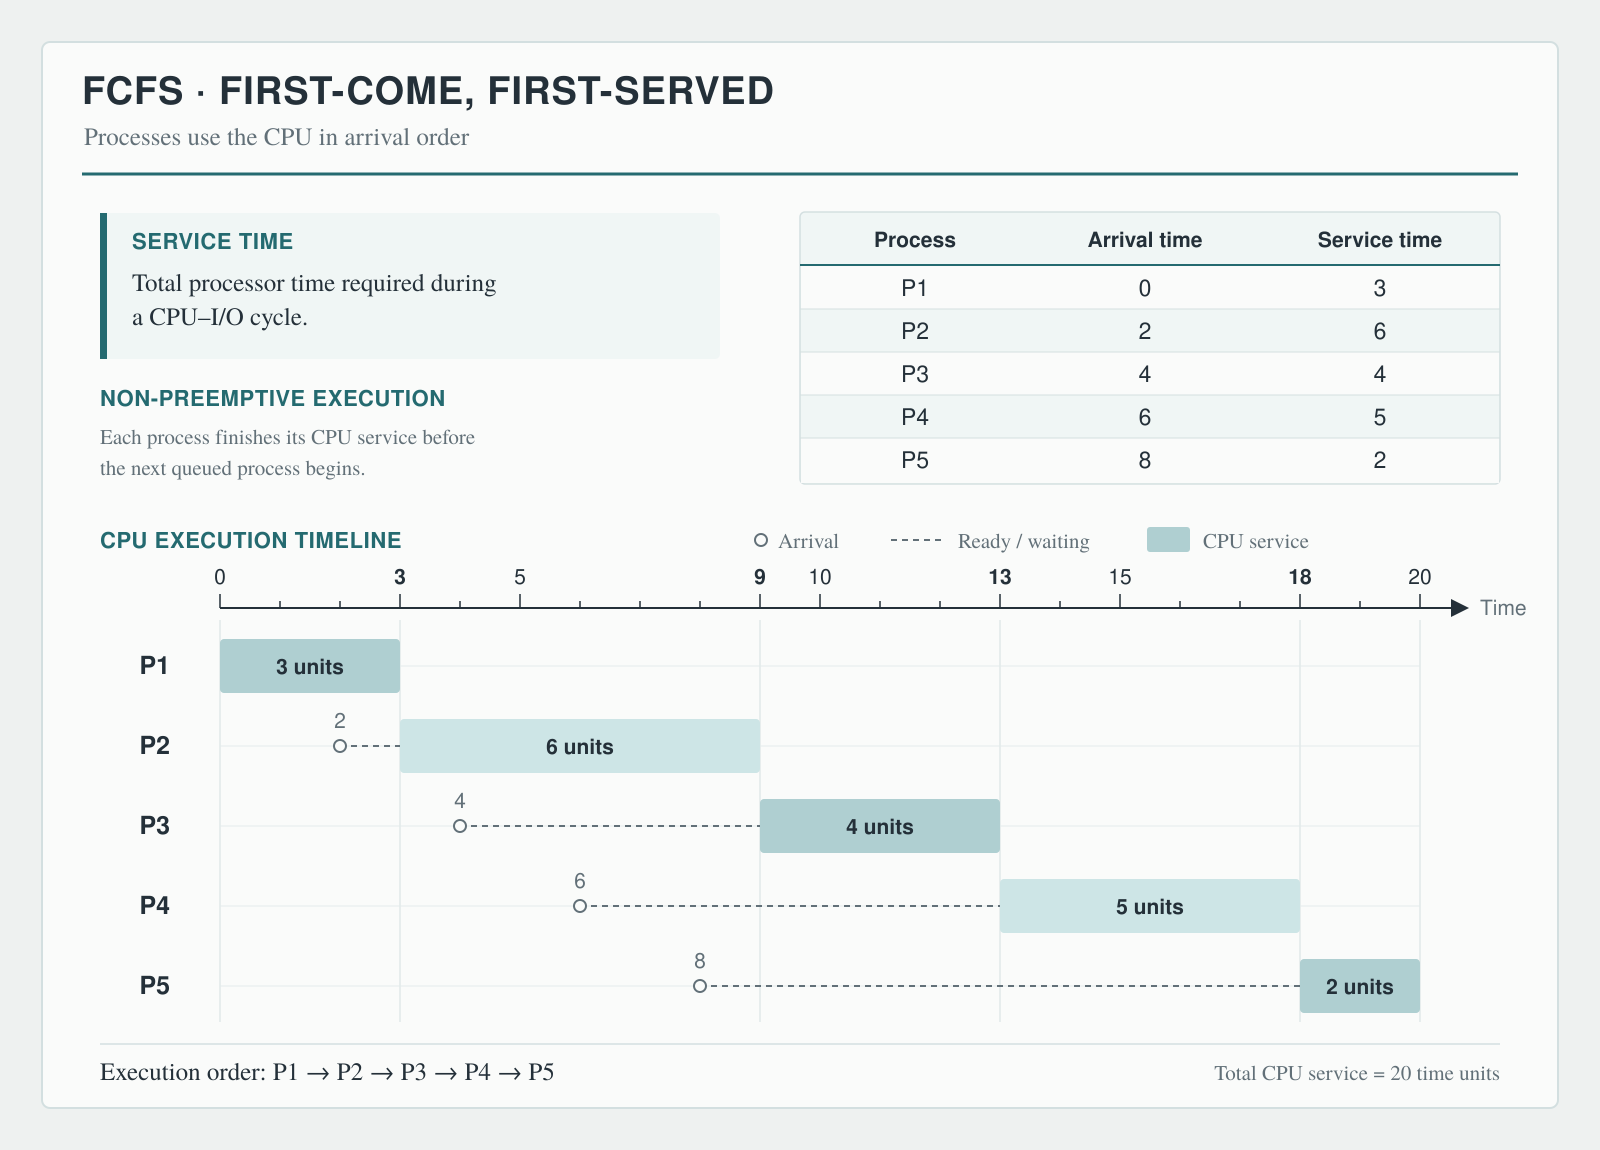
\includegraphics{figures/image-13749.png}}
\setlength{\fcfstoptrim}{0.434783\ht\fcfsimagebox}
\noindent\begin{minipage}{\linewidth}\centering
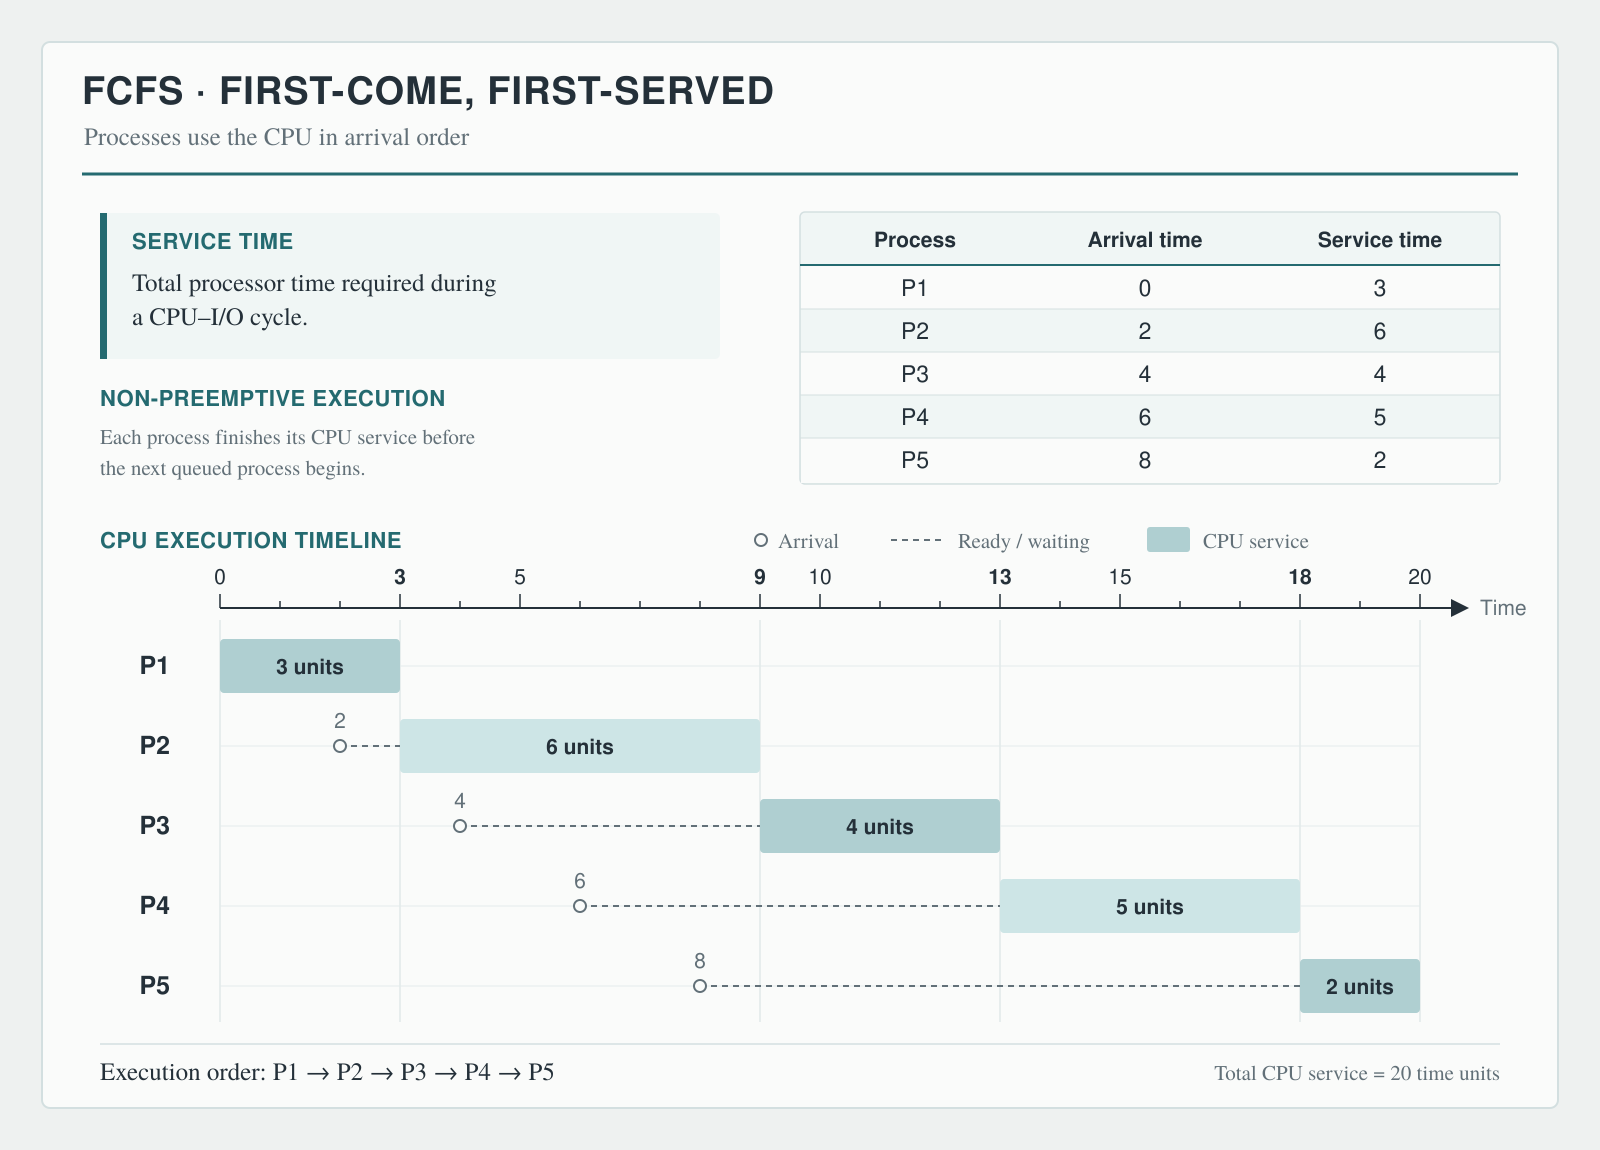
\includegraphics[width=\linewidth,height=70mm,keepaspectratio,trim=0 0 0 {\fcfstoptrim},clip]{figures/image-13749.png}\par
\end{minipage}\par\smallskip
\end{minipage}\par\smallskip


\Needspace{125pt}
\noteheading{3}{Time-sliced Scheduling (Round-robin)}





\Needspace{52pt}
\begin{multicols}{2}
\begin{itemize}
\item \begin{minipage}[t]{\linewidth}Each process runs for a fixed amount of time, and are run in a round-robin sequence\end{minipage}
\item \begin{minipage}[t]{\linewidth}Appropriate for regular multi-programming environments\end{minipage}
\item \begin{minipage}[t]{\linewidth}Has poor response time performance\end{minipage}
\end{itemize}
\end{multicols}



\textbf{Selection Mode:} FCFS\par

\textbf{Decision Mode}: Preemptive - a process is allowed to run until the time slice period has expired. Then a clock interrupt occurs, and the running process is put on a \code{READY} queue\par



Time quantum must \textgreater{}\textgreater{} than the time required to handle the clock interrupt and dispatching (\emph{context switch time}). Since this is overhead, the CPU will not waste time on the overhead and actually execute the application\par



\Needspace{52pt}
\begin{itemize}
\item I/O bound processes use the CPU for a time less than $\Delta q$ and is blocked waiting for the I/O
\item If $\Delta q$ is very, very large, then RR will turn into FCFS
\end{itemize}

\sourcefigure{image-13914.png}{85mm}

\noteheading{4}{Virtual RR}



Higher priority moves to AUX Q (IO interrupt tasks move to virtual RR), and gets preference over the main ready queue.\par



\sourcefigure{image-14342.png}{90mm}



\textcolor{red}{Look at Slide 58 - 60 and attempt problem.}\par




\end{document}
